\input{~/macro.tex}
% itemizeの変更
\renewcommand{\labelitemii}{$\circ$}
\renewcommand{\labelitemiii}{$\triangleright$}
\title{プラズマ中の波動}
\author{20B01392 松本侑真}
\date{\today}
\begin{document}
\maketitle
\begin{abstract}

\end{abstract}
\tableofcontents
\newpage

\section{概要}
プラズマ中の波動は、外部磁場が印加されている場合とそうでない場合などで沢山の種類に分類される。まずはプラズマ波の一覧を列挙する:
\begin{itemize}
	\item 縦波($\bm{k}\perp \bm{E}$)
	      \begin{itemize}
		      \item $\bm{B}_0 = 0$
		            \begin{itemize}
			            \item 電子プラズマ波
			            \item イオン音波
		            \end{itemize}
		      \item $\bm{B}_0 \neq 0$
		            \begin{itemize}
			            \item 高域混成振動($T=0$)
			            \item 低域混成振動
			            \item 静電イオンサイクロトロン波($\theta\approx \SI{90}{\deg}$であり、横波成分は必ず含まれる。)
		            \end{itemize}
	      \end{itemize}
	\item 横波($\bm{k}\varParallel\bm{E}$)
	      \begin{itemize}
		      \item $\bm{B}_0 = 0$
		            \begin{itemize}
			            \item プラズマ周波数$\omega_P$を遮断周波数とした$\omega > \omega_P$の通常の電磁波
		            \end{itemize}
		      \item $\bm{B}_0 =0 \wedge \bm{k}\perp \bm{B}_0$
		            \begin{itemize}
			            \item $\bm{E}_1 \varParallel \bm{B}_0$:正常波(O波)
			            \item $\bm{E}_1 \perp \bm{B}_0$:異常波(X波)
		            \end{itemize}
		      \item $\bm{B}_0 =0 \wedge \bm{k}\varParallel \bm{B}_0$
		            \begin{itemize}
			            \item L波とR波である円偏光の重ね合わせの電磁波
		            \end{itemize}
	      \end{itemize}
\end{itemize}

\newpage
\section{流体としてのプラズマの解析方法}
プラズマが流体みなせるための条件は
\begin{equation}
	\text{イオンや電子の平均自由行程}\ll\text{プラズマサイズ}
\end{equation}
が満たされることである。プラズマ中で荷電粒子が十分に衝突を繰り返し、Maxwell分布での平衡状態を達成することで温度が定義される。
\subsection{理想流体としてのプラズマの運動方程式}
単一荷電粒子の運動方程式は以下で与えられた:
\begin{equation}
	m\dv{\bm{v}(t)}{t} = q\qty{\bm{E} + \bm{v}\cross\bm{B}}\;。
\end{equation}
まず、衝突や熱運動がないと仮定する。このとき、流体要素中のすべての粒子は一緒に動き、粒子の平均速度$\bm{u}$は個々の粒子の速度$\bm{v}$に等しい。
したがって、流体の方程式は密度$n$をかけることによって得られる:
\begin{equation}
	mn\dv{\bm{u}(t)}{t} = qn\qty{\bm{E} + \bm{u}\cross\bm{B}}\;。
\end{equation}
しかし、このままでは扱いにくい。なぜなら、左辺の時間微分は粒子とともに動いている座標系(Lagrange座標系)で行わねばならないからだ。
この座標系では微小な流体要素の挙動のみを追うことができる。そのため、空間に固定された座標系(Euler座標系)に変換し、プラズマ全体の集団的挙動を解析できるようにする。
すなわち、あるEuler座標系からの位置ベクトル$\bm{x}$を用いて、プラズマの速度ベクトルの位置依存性を考慮する:
\begin{equation}
	\dv{\bm{u}(\bm{x},\,t)}{t} = \pdv{\bm{u}}{t} + \pdv{\bm{u}}{x_i}\dot{x}_i = \pdv{\bm{u}}{t} + \qty(\dot{\bm{x}}\cdot\grad)\bm{u}\;。
\end{equation}
ここで、固定された座標系から見たプラズマの位置ベクトルの時間変化$\dot{\bm{x}}$は流体の移動速度$\bm{u}$に他ならず、プラズマの運動方程式は以下のように記述される:
\begin{equation}
	mn\qty[\pdv{\bm{u}}{t} + \qty(\bm{u}\cdot\grad)\bm{u}] = qn\qty{\bm{E} + \bm{u}\cross\bm{B}}\;。
	\label{eq:ideal_eq}
\end{equation}
なお、左辺第二項は対流項と呼ばれるものである。

\subsection{流体に作用するマクロな力を考慮したプラズマの運動方程式}
熱運動や衝突を考慮しない式\eqref{eq:ideal_eq}で表される運動方程式では、流体にかかるマクロな力を考慮していない。流体全体の運動量変化を考えることで、マクロな力が加わった運動方程式が導出される。
まずは、簡単のために$x$方向の圧力変化を考える。粒子は微小時間$\varDelta t$の間に平均速度$\ev{v_x}$で$\varDelta x$の距離を進むとする。

$x = x_0$が中心であり、体積$\varDelta x\varDelta y\varDelta z$の流体要素に流入する運動量$P_+$は
\begin{equation}
	P_+ = \qty[\qty(\varDelta n\ev{v_x}\varDelta y\varDelta z) m\ev{v_x}]_{x_0-\varDelta x}\varDelta t
\end{equation}
と表される。ここで、$\varDelta n$は平均速度$\ev{v_x}$を持って流体要素に流入してくる粒子数であり、$\varDelta n = n/2$の関係がある。
なお、圧力が定義できているということは、粒子の速度分布はMaxwell分布になっていることを用いた。流体要素から流出する運動量$P_-$は
\begin{equation}
	P_- = \qty[\qty(\varDelta n\ev{v_x}\varDelta y\varDelta z) m\ev{v_x}]_{x_0}\varDelta t
\end{equation}
と表される。したがって、流体要素中の運動量変化は逆方向に進む粒子も考慮して、
\begin{equation}
	\frac{\varDelta P}{\varDelta t} = 2\frac{P_+ - P_-}{\varDelta t} =\varDelta y\varDelta z\frac{\qty[mn\ev{v_x^2}]_{x_0-\varDelta x}-\qty[mn\ev{v_x^2}]_{x_0}}{\varDelta t}
\end{equation}
と表される。$\varDelta t\to 0$の極限を取ると、
\begin{equation}
	\pdv{P}{t} = -m\pdv{x}\qty(n\ev{v_x^2})\varDelta x\varDelta y\varDelta z
\end{equation}
となる。これが流体自身の正味の圧力変化と等しくなるため、
\begin{equation}
	\pdv{t}(nmu_x)\varDelta x\varDelta y\varDelta z = -m\pdv{x}\qty(n\ev{v_x^2})\varDelta x\varDelta y\varDelta z
	\label{eq:P_henka}
\end{equation}
が成立する。ここで、粒子の速度を流体速度$u_x$と熱速度$v_{xT}$に分離する:
\begin{equation}
	v_x = u_x + v_{xT},\quad \ev{u_x} = u_x,\quad \ev{v_{xT}} = 0,\quad\frac{1}{2}m\ev{v_{xT}^2} = \frac{1}{2}k_\text{B}T\;。
\end{equation}
このとき、式\eqref{eq:P_henka}は

\begin{gather}
	\pdv{t}(mnu_x)  = -m\pdv{x}\qty[n\ev{u_x^2 + 2u_xv_{xT} + v_{xT}^2}] = -m\pdv{x}\qty[n\qty(u_x^2 + \frac{k_\text{B}T}{m})] \\
	\therefore\; mn\pdv{u_x}{t} + mu_x\pdv{n}{t} = -mu_x\pdv{x}(nu_x) - mnu_x\pdv{u_x}{x} - \pdv{x}\qty(nk_{\text{B}}T)
\end{gather}
と計算できる。\footnote{$nu_x^2 = (nu_x)\cdot u_x$とみなして積の微分法を用いた。}
また、左辺が質量保存則
\begin{equation}
	\pdv{n}{t} + \pdv{x}(nu_x) = 0
\end{equation}
を用いて、流体の圧力を$P = nk_{\text{B}}T$と置くと、最終的に
\begin{equation}
	mn\pdv{u_x}{t} = - mnu_x\pdv{u_x}{x} - \pdv{P}{x}
\end{equation}
となる。したがって、$y,\,z$方向でも同様の議論が成立し、理想的な場合の運動方程式と合わせて
\begin{equation}
	mn\qty[\pdv{\bm{u}}{t} + \qty(\bm{u}\cdot\grad)\bm{u}] = qn\qty{\bm{E} + \bm{u}\cross\bm{B}} - \grad{P}
\end{equation}
となる。

\subsection{流体プラズマを記述する方程式群}
\subsubsection{運動方程式}
\begin{equation}
	mn\qty[\pdv{\bm{u}}{t} + \qty(\bm{u}\cdot\grad)\bm{u}] = qn\qty{\bm{E} + \bm{u}\cross\bm{B}} - \grad{P}
\end{equation}
\subsubsection{Maxwell方程式}
電荷密度$\sigma  = n_iq_i + n_eq_e$、電流密度$\bm{j} = n_iq_i\bm{v}_i + n_eq_e\bm{v}_e$とおける:
\begin{align}
	\div{\bm{E}}     & = 4\pi\qty(n_iq_i + n_eq_e)                                 \\
	\curl{\bm{E}}    & = -\dot{\bm{B}}                                             \\
	\div{\bm{B}}     & = 0                                                         \\
	c^2\curl{\bm{B}} & = 4\pi\qty(n_iq_i\bm{v}_i + n_eq_e\bm{v}_e)  + \dot{\bm{E}}
\end{align}

\subsubsection{連続の式}
体積$V$中の粒子の総数$N$は$V$を囲む表面$S$を横切る正味の粒子の流束がある場合にのみ変化する。粒子の流束密度は$n\bm{u}$であるため、Stokesの定理により、
\begin{equation}
	\pdv{N}{t} = \int_V\pdv{n}{t}dV = -\oint_S (n\bm{u})\cdot d\bm{S} = -\int_V \div\qty(n\bm{u})dV
\end{equation}
が任意の$V$で成立する。したがって、連続の式は以下のようになる:
\begin{equation}
	\pdv{n}{t} + \div{(n\bm{u})} = 0\;。
\end{equation}

\subsubsection{状態方程式}
圧力$p$と粒子数密度$n$を関係付ける熱力学の状態方程式を扱う:
\begin{equation}
	p = C\rho^\gamma\;。
\end{equation}
ここで、$C$は定数で$\gamma$は比熱比$C_p/C_V$である。したがって、
\begin{equation}
	\frac{\grad{p}}{p} = \gamma\frac{\grad{n}}{n}
\end{equation}
となり、等温圧縮では
\begin{equation}
	\grad{p} = \grad\qty(nk_{\text{B}}T) = k_{\text{B}}T\grad{n}
\end{equation}
が成立するため、明らかに$\gamma=1$となる。断熱圧縮に対しては、自由度$N$に対して
\begin{equation}
	\gamma = (2+N)/N
\end{equation}
が成立する。
\subsection{外部磁場に対する流体ドリフトについて}
\subsubsection{外部磁場に垂直な流体ドリフト}
流体要素はたくさんの粒子から成っているため、個々の粒子の旋回中心が外部磁場$\bm{B}$に垂直な方向にドリフトをすれば、流体も$\bm{B}$に垂直な方向にドリフトされることが期待される。
しかし、実際は$\grad{\bm{B}}$ドリフトは流体中に存在せず、圧力勾配が存在する場合には流体全体のドリフト運動が生じることを示す。

まず、プラズマ中の粒子の運動方程式
\begin{equation}
	mn\qty[\pdv{\bm{v}}{t} + \qty(\bm{v}\cdot\grad)\bm{v}] = qn\qty{\bm{E} + \bm{v}\cross\bm{B}} - \grad{P}
\end{equation}
において、$\bm{v} = e^{i(\bm{k}\cdot\bm{r} - wt)}$とおく。また、磁場に垂直な成分$\bm{v}_{\perp}$の運動を考えることにする。サイクロトロン角周波数$\omega_c = qB/m$を用いると、
\begin{equation}
	\qty|\frac{mn\pdv*{\bm{v}_\perp}{t}}{qn\bm{v}_{\perp}B}| = \qty|\frac{m\omega}{qB}| \approx \frac{\omega}{\omega_c}
\end{equation}
となるため、サイクロトロン運動の時間スケールより遅いドリフトであれば$\pdv*{\bm{v}_{\perp}}{t}$は無視できる。
また、後にわかることであるが、対流項は$\qty(\bm{v}_{\perp}\cdot\grad)\bm{v}_{\perp} = 0$となるため、無視して計算を行う。
$\bm{B}$との外積を作ることで、運動方程式は以下のように変形できる:
\begin{equation}
	\begin{aligned}
		0 & = qn\qty[\bm{E}\cross\bm{B} + \qty(\bm{v}_{\perp}\cross\bm{B})\cross\bm{B}] - \grad{P}\cross\bm{B}                 \\
		  & = qn\qty[\bm{E}\cross\bm{B} + \bm{B}\qty(\bm{v}_{\perp}\cdot\bm{B}) - \bm{v}_{\perp}B^2] - \grad{P}\cross\bm{B}\;。
	\end{aligned}
\end{equation}
したがって、
\begin{equation}
	\bm{v}_{\perp} = \frac{\bm{E}\cross\bm{B}}{B^2} - \frac{\grad P\cross\bm{B}}{qnB^2} \coloneqq \bm{v}_\text{E} + \bm{v}_\text{D}
\end{equation}
と求まる。ここで、
\begin{equation}
	\bm{v}_\text{E} = \frac{\bm{E}\cross\bm{B}}{B^2}\qquad\text{$\bm{E}\cross\bm{B}$ドリフト}
\end{equation}
\begin{equation}
	\bm{v}_\text{D} =  - \frac{\grad P\cross\bm{B}}{qnB^2} \qquad\text{反磁性ドリフト}
\end{equation}
である。反磁性ドリフトによってプラズマが反磁性の性質を持つことを図解する。図\ref{fig:entyu}は、円柱プラズマ内に磁場が印加されており、中心軸方向に圧力勾配が存在する場合を表している。
\begin{figure}[H]
	\centering
	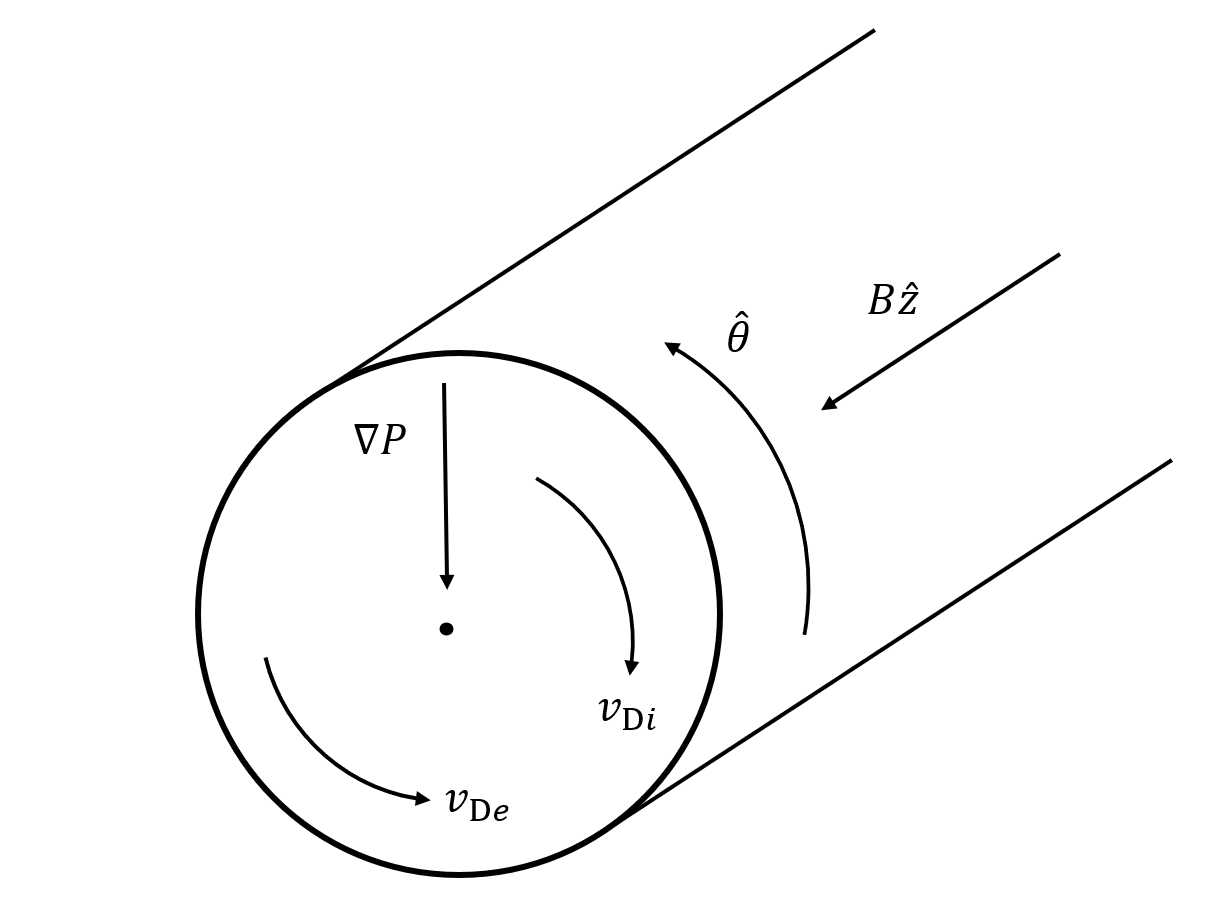
\includegraphics[width=0.7\linewidth]{entyuu_plasma.png}
	\caption{円柱プラズマ内の反磁性ドリフト}
	\label{fig:entyu}
\end{figure}
$\grad{P}\propto -\hat{r},\,\bm{B}\propto \hat{z}$であるため、$\bm{v}_{\text{D}}\propto -\hat{\theta}$となる。
すなわち、イオンの反磁性ドリフト、電子の反磁性ドリフトそれぞれが外部磁場$\bm{B}$を打ち消す方向の円電流を生むことがわかる。
そのため、プラズマ内に同じ方向の電流$\bm{j}_{\text{D}}$が生じることがわかる。その値はプラズマ近似$n_i=n_e=n$の元で
\begin{equation}
	\bm{j}_{\text{D}} = ne(\bm{v}_{\text{D}i} - \bm{v}_{\text{D}e}) = \qty(k_{\text{B}}T_i + k_{\text{B}}T_e)\frac{\bm{B}\cross\grad{n}}{B^2}
\end{equation}
である。
最後に、対流項が磁場に垂直な成分を持たないことを示す。
\begin{equation}
	\bm{v}\cdot\grad =
	\begin{pmatrix}
		v_r & v_\theta & v_z
	\end{pmatrix}
	\begin{pmatrix}
		\pdv{r}                 \\
		\frac{1}{r}\pdv{\theta} \\
		\pdv{z}
	\end{pmatrix}
\end{equation}
であることと、$\bm{v}_{\text{D}} = v(r)\hat{\theta}$と表されることより、
\begin{equation}
	\qty(\bm{v}_{\text{D}}\cdot\grad)\bm{v}_{\text{D}} = \qty(v(r)\frac{1}{r}\pdv{\theta})v(r)\hat{\theta} = 0
\end{equation}
となる。

\subsubsection{外部磁場に平行な流体ドリフト}

\newpage
\section{横波}
\subsection{電子プラズマ波}
\subsection{イオン音波}
\subsection{高域混成振動}
\subsection{低域混成振動}
\subsection{静電イオンサイクロトロン波}

\section{縦波}
\subsection{外部磁場がない場合}
\subsection{正常波}
\subsection{異常波}
\subsection{外部磁場と波数ベクトルが平行な場合}

\end{document}